\documentclass[a4paper,titlepage,10pt]{article}

\usepackage[T1]{fontenc}
\usepackage[utf8]{inputenc}
\usepackage{polski}

\usepackage{enumerate}
\usepackage{amssymb}
\usepackage{amsmath}
\usepackage[pdftex]{graphicx}
\usepackage{tikz}
\usepackage[colorlinks=true,linkcolor=blue]{hyperref}
\usepackage{anysize}

\usepackage{lastpage}
\usepackage{fancyhdr}

\usepackage[a4paper, top=2.5cm, bottom=2.5cm, left=2cm, right=2cm]{geometry}
\linespread{1.3}

\title{\huge Symulacja układu planetarnego na GPU\\ przy użyciu CUDA i OpenGL\\\small Dokumentacja biznesowa}
\author{Daniel Kłobuszewski\and Jakub Kotur}

\begin{document}
	\maketitle
	
	\pagestyle{fancyplain}
%        \fancyhf{}
	\cfoot{\thepage/\pageref{LastPage}}

%        \marginsize{1cm}{1cm}{2.5cm}{2.5cm}

	\begin{figure}[h]
	\centering
\begin{tabular}{|p{.1\textwidth}|p{.04\textwidth}|p{.1\textwidth}|p{.1\textwidth}|p{.206\textwidth}|p{.1\textwidth}|}
	\hline
	\multicolumn{6}{|l|}{Metryka dokumentu} \\
	\hline
	Projekt & \multicolumn{2}{l|}{Symulacja układu planetarnego na GPU } &
	Firma & \multicolumn{2}{l|}{Politechnika Warszawska} \\
	&  \multicolumn{2}{l|}{przy użyciu CUDA i OpenGL} & &  \multicolumn{2}{l|}{} \\
	\hline
	Nazwa & \multicolumn{5}{l|}{Dokumentacja techniczna} \\
	\hline
	Temat & \multicolumn{5}{l|}{Specyfikacja techniczna projektu} \\
	\hline
	Autor & \multicolumn{5}{l|}{Daniel Kłobuszewski, Jakub Kotur} \\
	\hline
	Plik & \multicolumn{5}{l|}{tech.pdf} \\
	\hline
	Nr wersji & 06 & Status & Finalny & Data\par sporządzenia & 2010-10-09 \\
	\hline
	Streszczenie & \multicolumn{5}{p{11cm}|}{Celem dokumentu jest zdefiniowanie
		technicznych wymagań Projektu.} \\
	\hline
	Zatwierdził & \multicolumn{3}{l|}{ } &
	Data ostatniej\par modyfikacji & 2010-10-12 \\
	\hline
\end{tabular}

	\label{tab:metric}
\end{figure}


	%\newpage
	\begin{figure}[h]
	\centering

\begin{tabular}{|p{.075\textwidth}|p{.1\textwidth}|p{.2\textwidth}|p{.522\textwidth}|}
	\hline
	\multicolumn{4}{|l|}{Historia zmian dokumentu} \\
	\hline
	Wersja & Data & Kto & Opis \\
	\hline
	0.1 & 2011-01-02 & Jakub Kotur &
	Określenie podstawowej struktury dokumentu \\
	\hline
	0.2 & 2011-01-04 & Jakub Kotur &
	Dodanie opisów dziłania oraz zmian \\
	\hline
	1.0 & 2011-01-04 & Daniel Kłobuszewski &
	Poprawki ortograficzne i stylistyczne \\
	\hline
\end{tabular}

	\label{tab:hist}
\end{figure}



%        \marginsize{2cm}{2cm}{2.5cm}{2.5cm}
	\tableofcontents
	\newpage

	\paragraph{}
Poniższy dokument stanowi podsumowanie projektu, pisanego w ramach przedmiotu Projekt Zespołowy, na wydziale Matematyki i Nauk Informacyjnych Politechniki Warszawskiej w semestrze zimowym 2010/2011.

\paragraph{}
Opisujemy w nim zasady działania głównych modułów, różnice w stosunku do specyfikacji oraz wnioski z testów akceptacyjnych. Znajduje się tutaj także krótka instrukcja obsługi programu, która pozwoli zapoznać się z nim każdej osobie, która wcześniej nie miała z naszą aplikacją styczności.

	\section{Przypadki uzycia}\label{sec:usecase}

\paragraph{}

Poniższy diagram przedstawia przypadki użycia aplikacji przez użytkownika. Ponieważ najważniejszym elementem aplikacji są obliczenia na karcie graficznej, oraz wyświetlanie ich wyników w przyjaznej dla oka formie, główną aktywnością użytkownika jest oglądanie efektów obliczeń i cieszenie oka efektami specjalnymi. Jednak aby aplikacja była choć trochę funkcjonalna, użytkownikowi umożliwione będzie podstawowa kontrola symulacji.

\begin{figure}[h]
	\centering
	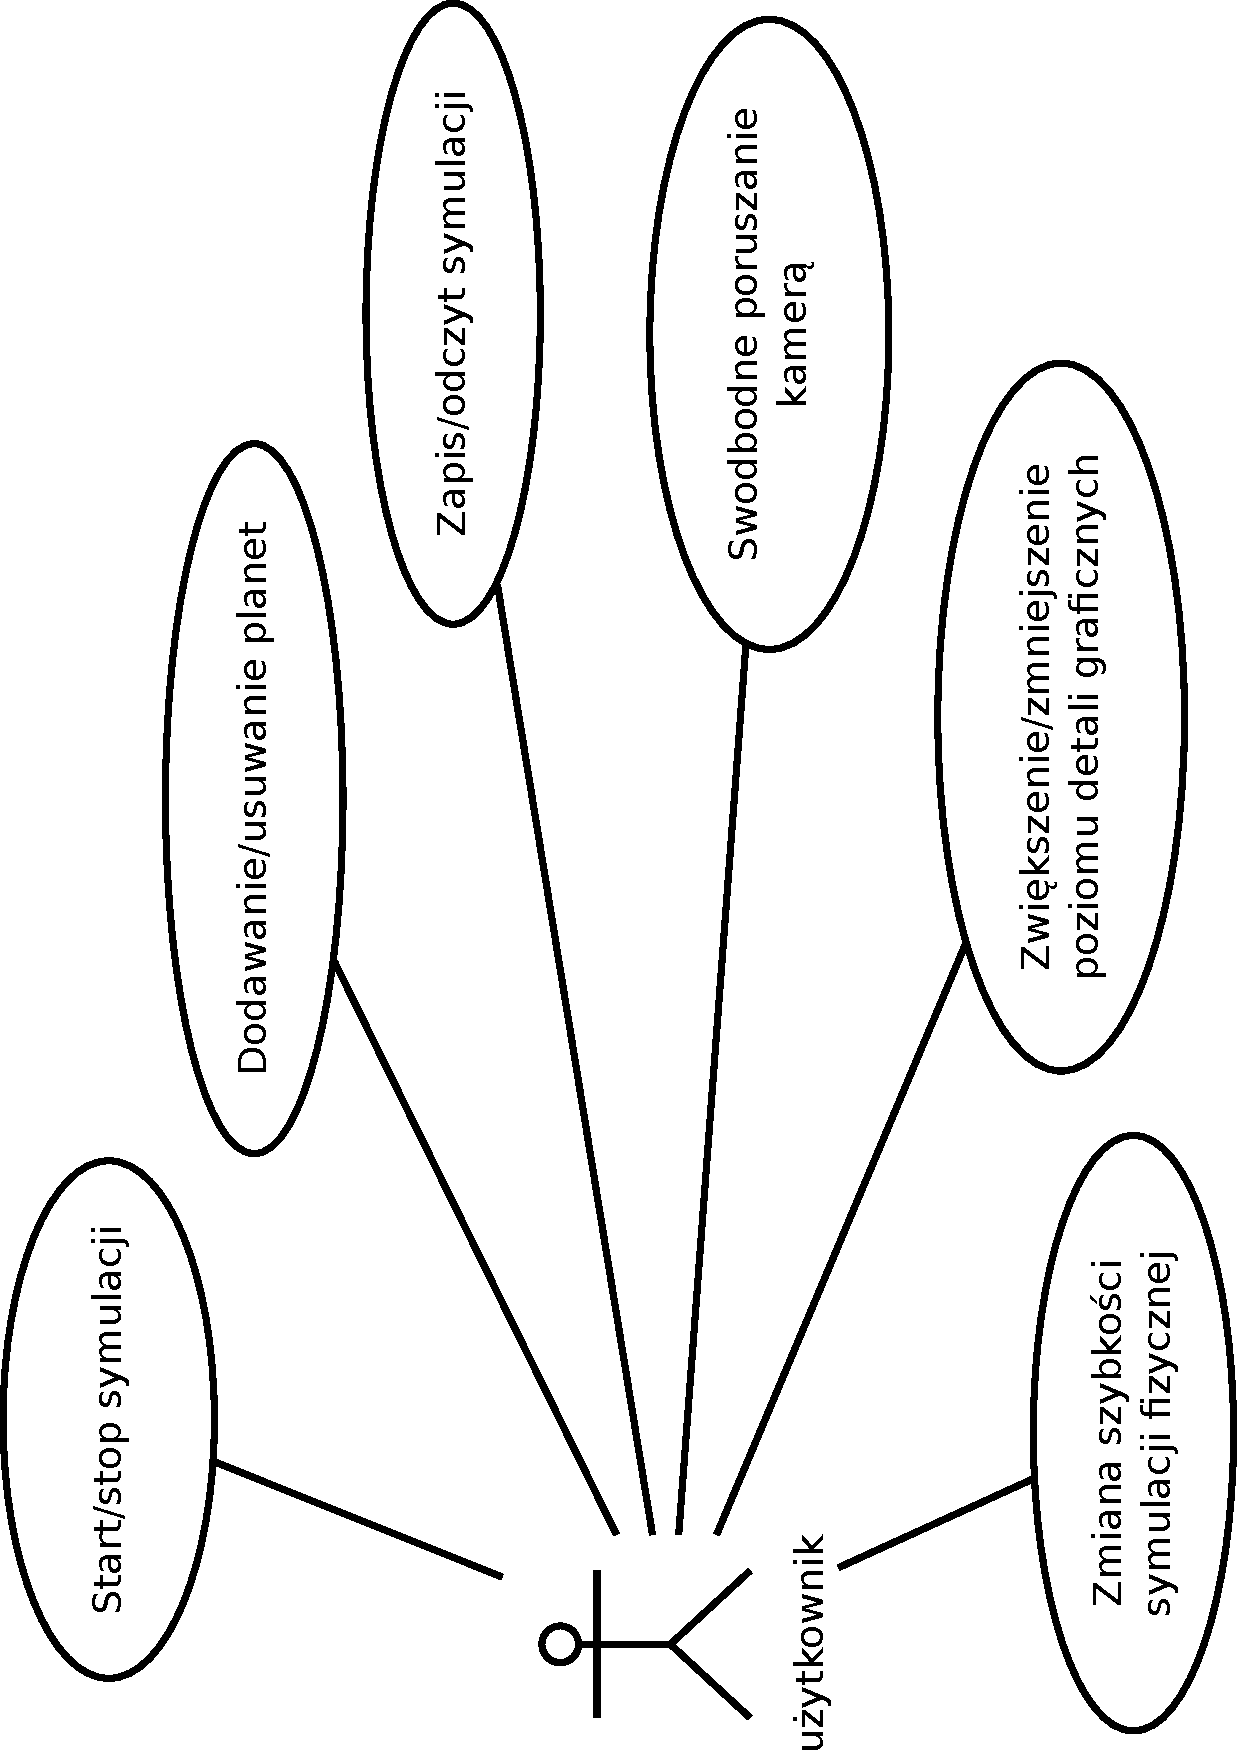
\includegraphics[width=0.5\textwidth,angle=-90]{use-case.pdf}
	\caption{Diagram przypadków użycia}
	\label{fig:use-case}
\end{figure}

\paragraph{}

Znaczenie poszczególnych przypadków użycia dla aplikacji jest następujące:

\begin{description}
	\item[Start/stop symulacji] - aplikacja powinna przewidywać możliwość zatrzymania i wznowienia symulacji fizycznej, nie blokując przy tym możliwości poruszania kamera. W trybie pauzy powinna być również możliwość dodawania/usuwania planet.
	\item[Dodawanie/usuwanie planet] - aby dać użytkownikowi możliwość budowania własnych układów, aplikacja powinna pozwalać na usuwanie planet uczestniczących w aktualnej symulacji, oraz na dodawanie nowych planet, nadając im masę, pozycje, oraz prędkość początkowa. Wygodnym sposobem ustawiania nowej planety jest używanie myszki, dla ustalenia pozycji, oraz prędkości początkowej.
	\item[Zapis/odczyt symulacji] - aplikacja powinna pozwalać na wczytywanie wcześniej zdefiniowanych układów, ponieważ uzyskanie stabilnego układu planetarnego nie jest rzeczą prostą. Jeśli jednak sie to uda, powinna być również możliwość zapisania aktualnego stanu symulacji.
	\item[Swobodne poruszanie kamera] - swobodna kamera oznacza, ze można przesuwać ja w dowolnym kierunku, tak aby była możliwość ustawienia jej w dowolnej pozycji, oraz można ja obracać w dowolna stronę. Na przesuwnie kamery najwygodniej pozwolić za pomocą klawiszy klawiatury, natomiast obroty najwygodniej realizuje sie poprzez ruch myszki.
	\item[Zmiana poziomu detali graficznych] - w zależności od mocy karty graficznej na maszynie wywołującej program, powinna być możliwość ustawienia szczegółowości prezentowanej symulacji. Miedzy innymi można sterować ilością wierzchołków składających sie na obiekt (teselacja), rozdzielczością oraz sposobem mapowania tekstur, ilością prezentowanych efektów specjalnych, ilością gwiazd (źródeł światła).
	\item[Zmiana szybkości symulacji fizycznej] - w zależności od możliwości jednostki graficznej na której dokonywane są obliczenia fizyczne, można ustawić więcej, bądź mniej klatek fizycznych na jedna klatkę graficzna, tak aby uzyskać tak samo dokładną symulacje w krótszym czasie.
\end{description}


	\section{Harmonogram}\label{sec:harmonogram}

\paragraph{}

Harmonogram prac przedstawiony jest poniżej wraz z opisami poszczególnych zadań. Zadania podzielone są tematycznie.

\subsection{Grafika}

\begin{description}
	\item[Wyświetlanie planet] \hfill \\
	Celem tego zadania jest stworzenie podstawowego świata 3D do wizualizacji symulacji. W skład zadania wchodzi dynamiczne generowanie modelu kuli na zadanym poziomie szczegółowości oraz jego reprezentacja w postaci zrozumialej przez jednostkę graficzną.
	\item[Teksturowanie planet] \hfill \\
	Zadanie to polega na wygenerowaniu współrzędnych tekstury zgodnych z modelem 3D planety i przekazanie tekstur oraz ich współrzędnych na jednostkę graficzną.
	\item[Dynamiczna zmiana szczegółowości planet] \hfill \\
	W zależności od odległości kamery od planety, powinna być ona wyświetlana na rożnym poziomie dokładności. W szczególności, blisko kamery powinna być to możliwie dokładna kula, natomiast w dużej odległości, powinna sie stawać punktem, a nawet całkiem zanikać.
	\item[Efekt atmosfery] \hfill \\
	Aby nadać planetom bardziej realistyczny wygląd, powinno się je otoczyć półprzezroczystą poświatą wyglądającą jak atmosfera.
	\item[Efekt warkocza komety] \hfill \\
	Niektóre obiekty będą kometami. Będą wyróżniać się charakterystycznym ogonem, stanowiącym chmurę cząsteczek wygenerowanych przez moduł fizyczny.
	\item[Oświetlenie] \hfill \\
	Zastosujemy oświetlenie rozproszone. Dodatkowo punktowym źródłem światła będą gwiazdy. Planety powinny być oświetlane przez gwiazdy, które są dość blisko. Gwiazdy będące daleko powinny być pomijane przy obliczaniu koloru planety. Najlepszy w tym celu będzie model oświetlenia Phonga.
	\item[Efekt gwiazd] \hfill \\
	Gwiazdy są specyficznymi obiektami z punktu widzenia oświetlenia, ponieważ same emitują światło. Dla takich obiektów nie należy obliczać oświetlenia, natomiast nadać im realistyczny kolor.
\end{description}

\subsection{Interfejs uzytkownika}

\begin{description}
	\item[Sterowanie symulacją] \hfill \\
	Interfejs użytkownika powinien umożliwiać wszystkie operacje uwzględnione w diagramie przypadków użycia. Ponieważ nie ma ich dużo i są niezależne, dla każdej opcji będzie przewidziany oddzielny przycisk widoczny w głównym oknie symulacji.
	\item[Interaktywna kamera] \hfill \\
	Kamera będzie wolna. Oznacza to, że użytkownik przy pomocy myszki i klawiszy może dowolnie poruszać sie po świecie 3D, w tym przypadku po kosmosie.
\end{description}

\subsection{Symulacja fizyczna}

\begin{description}
	\item[Obliczanie nowych pozycji planet] \hfill \\
	Silnik fizyczny musi na bieżąco, na podstawie mas planet i ich położeń względem siebie, obliczać prędkości oraz nowe położenia. 
	\item[Detekcja i obsługa kolizji] \hfill \\
	Może się zdarzyć, że dwie planety znajdą się zbyt blisko siebie. Żeby nie dochodziło do "przenikania" planet przez siebie nawzajem, trzeba rozwiązać problem kolizji. Zderzające się planety będą mogły rozpaść się na więcej obiektów lub stworzyć jeden, większy.
	\item[Klasteryzacja planet] \hfill \\
	Aby zmniejszyć ilość obliczeń pozycji planet, będą one grupowane w klastry. Planety będą oddziaływać na siebie nawzajem wewnątrz klastra. Oddziaływanie z planetami spoza klastra odbywać się będzie pośrednio, poprzez wyliczenie oddziaływań uśrednionych.

\end{description}

\subsection{Inne}

\begin{description}
	\item[Serializacja i deserializacja układów] \hfill \\
	Aplikacja będzie umożliwiała użytkownikowi zapisywanie/wczytywanie układów planetarnych. Każdy układ będzie zapisywany do oddzielnego pliku z niezbędnymi informacjami o każdej planecie: pozycji, prędkości, masie, wielkości i rodzaju. Do opisu w pliku nie będzie użyty język XML, gdyż znacznie zwiększa on ilość miejsca potrzebną do zapisu. Dane będą zapisywane binarnie.
	\item[Reprezentacja planet w pamięci] \hfill \\
	Obiekt planety będzie złożony - czym innym jest planeta dla fizyki, czym innym dla grafiki. Potrzebne będą struktury danych pozwalające na optymalne wykorzystanie pamięci RAM karty graficznej - trzeba bowiem uniknąć przesyłania danych pomiędzy pamięcią karty a RAM'em komputera.
	\item[Generowanie cząsteczek] \hfill \\
	Chmury cząsteczek składające się na ogon komety także będą obliczane na karcie graficznej, przez aplikację, na podstawie kilku ostatnich położeń obiektu.
\end{description}

\begin{landscape}
\begin{figure}[ht]
	\begin{gantt}{25}{15}
		\begin{ganttitle}
			\titleelement{Październik}{4}
			\titleelement{Listopad}{4}
			\titleelement{Grudzień}{4}
			\titleelement{\footnotesize Święta}{1}
			\titleelement{Styczeń}{2}
		\end{ganttitle}
		\begin{ganttitle}
			\numtitle{40}{1}{52}{1}
			\numtitle{1}{1}{2}{1}
		\end{ganttitle}
		\ganttgroup{\bf{Projekt}}{0}{3}
		\ganttbar{Dokumentacja biznesowa}{0}{1}
		\ganttbar{Dokumentacja techniczna}{1}{2}
		\ganttgroup{\bf{Grafika}}{3}{9}
		\ganttbar[pattern=]{Wyświetlanie planet}{3}{1}
		\ganttbar[pattern=]{Teksturowanie planet}{6}{1}
		\ganttbar[pattern=]{Oświetlenie}{7}{2}
		\ganttbar[pattern=]{Efekt gwiazd}{8}{1}
		\ganttbar[pattern=]{Dynamiczna zmiana szczegółowości planet}{9}{2}
		\ganttbar[pattern=]{Efekt atmosfery}{10}{1}
		\ganttbar[pattern=]{Efekt warkocza komety}{11}{1}
		\ganttgroup{\bf{Interfejs użytkownika}}{4}{2}
		\ganttbar[pattern=]{Sterowanie symulacją}{4}{2}
		\ganttbar[pattern=]{Interaktywna kamera}{4}{1}
		\ganttgroup{\bf{Symulacja fizyczna}}{3}{9}
		\ganttbar[color=white]{Obliczanie nowych pozycji planet}{3}{3}
		\ganttbar[color=white]{Detekcja i obsługa kolizji}{6}{3}
		\ganttbar[color=white]{Klasteryzacja planet}{9}{3}
		\ganttgroup{\bf{Inne}}{0}{0}
		\ganttbar[color=white]{Serializacja i deserializacja układów}{4}{1}
		\ganttbar{Reprezentacja planet w pamięci}{2}{1}
		\ganttbar[color=white]{Generowanie cząsteczek}{10}{1}
		\ganttbar{Poprawki}{13}{2}
	\end{gantt}
	\caption{Wykres Gantta}
	\label{gantt}
\end{figure}
%  \scalebox{0.8}{
%  \begin{gantt}[xunitlength=0.5cm,fontsize=\small,titlefontsize=\small,drawledgerline=true]{10}{48}
  \end{landscape}

	\section{GUI}\label{sec:gui}

\begin{figure}[h]
	\centering
	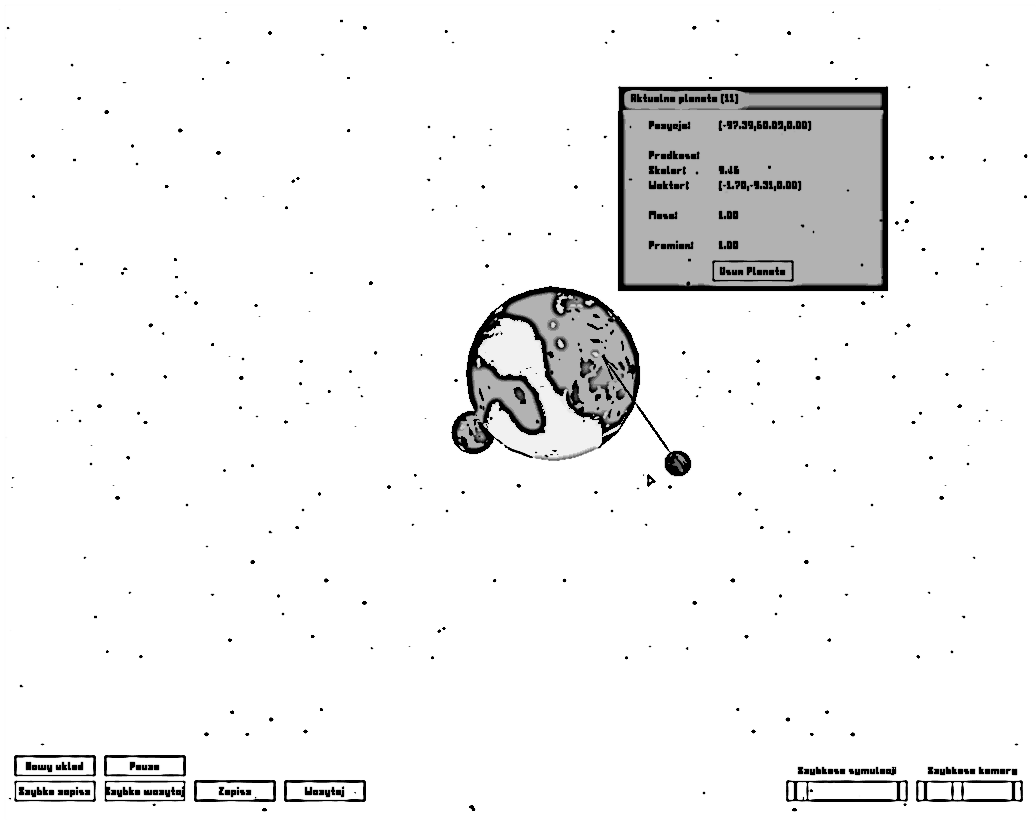
\includegraphics[width=0.9\textwidth]{gui.png}
	\caption{Prototyp interfejsu}
	\label{fig:gui}
\end{figure}



\end{document}

